\chapter{Quality Assurance Framework}
\markboth{Quality Assurance Framework}{}

\section{Introduction}

This chapter presents the quality assurance framework used during the software testing process at SeekMake.

It covers quality assurance vs testing, the Scrum methodology, the integration of DevOps, testing strategy, testing types, testing tools, and testing techniques used to ensure the quality of the software.

\section{Quality Assurance vs Testing}

While people often use the terms “testing” and “quality assurance” (QA) interchangeably, testing and QA
are not the same \cite{istqbctfl4.0.1}:

\subsection{Quality Assurance}

QA is a process-oriented, preventive approach that focuses on the implementation and improvement of
processes. It works on the basis that if a good process is followed correctly, then it will generate a good
product. \cite{istqbctfl4.0.1}

QA at SeekMake guided the testing process by defining the testing strategy, planning the testing activities, and ensuring that the testing activities were aligned with the sprint goals.

\subsection{Software Testing}

Testing is a product-oriented, corrective approach that focuses on those activities supporting the
achievement of appropriate levels of quality. \cite{istqbctfl4.0.1}

Testing at SeekMake was carried out to identify and fix defects\footnote{A defect is an error, flaw, failure, or fault in a computer program that causes it to produce an incorrect or unexpected result, or to behave in unintended ways} in the web application. This corrective approach was complemented by QA activities that focused on process improvement and defect prevention.

\subsection{Differences and Complementarity}

Test results are used by QA and testing. In testing they are used to fix defects, while in QA they provide
feedback on how well the development and test processes are performing. \cite{istqbctfl4.0.1}

\section{Scrum Methodology}

At SeekMake, the testing process was aligned with the Scrum methodology.

\subsection{Scrum Overview}

Scrum helps people and teams deliver value incrementally in a collaborative way. As an agile framework, Scrum provides just enough structure for people and teams to integrate into how they work, while adding the right practices to optimize for their specific needs. \cite{scrum}

At SeekMake, Scrum was used to manage the testing process, ensuring that the testing activities were aligned with the sprint goals and that the testing process was integrated with the development activities.
\subsection{Scrum Team}

The fundamental unit of Scrum is a small team of people, a Scrum Team. The Scrum Team consists of one Scrum Master, one Product Owner, and Developers. \cite{scrum}

At SeekMake, the Scrum Team consisted of developers (including QA testers and UX/UI designers), a product owner, and a Scrum master.
\subsubsection{Scrum Master}

the Scrum Master is accountable for establishing Scrum. They do this by helping everyone understand Scrum theory and practice, both within the Scrum Team and the organization while serving the Scrum Team as well as the larger organization. \cite{scrum}

\subsubsection{Product Owner}
The Product Owner is accountable for maximizing the value of the product resulting from the work of the Scrum Team. How this is done may vary widely across organizations, Scrum Teams and individuals. \cite{scrum}

\subsubsection{Developers}
Developers are the people on the Scrum Team that are committed to creating any aspect of a usable Increment each Sprint.\cite{scrum}

\subsection{Scrum Events}

Each event in Scrum is a formal opportunity to inspect and adapt Scrum artifacts. These events are specifically designed to enable the transparency required. Failure to operate any events as prescribed results in lost opportunities to inspect and adapt. Events are used in Scrum to create regularity and to minimize the need for meetings not defined in Scrum. \cite{scrum}

\subsubsection{Sprints}

Sprints are fixed length periods of work that last one month or less to create consistency and ensure short iterations for feedback in order to inspect and adapt both how work is done and what is being worked on. \cite{scrum}

At SeekMake, sprints lasted two weeks and were used to define the scope of the testing activities, assign tasks to team members, and estimate the effort required to complete the testing activities.

\subsubsection{Sprint Planning}

Sprint Planning initiates the Sprint by laying out the work to be performed for the Sprint. This resulting plan is created by the collaborative work of the entire Scrum Team. \cite{scrum}

\subsubsection{Daily Scrum}

The Daily Scrum (or daily Stand-Up) is a 15-minute event for the Developers of the Scrum Team. To reduce complexity, it is held at the same time and place every working day of the Sprint. \cite{scrum}

At SeekMake, daily stand-ups were used to share updates, collaborate on testing activities, and resolve issues.

\section{Integration of DevOps}
At SeekMake, the testing process was integrated with DevOps practices to ensure that the testing activities were aligned with the development activities.

\subsection{DevOps Overview}

DevOps is an organizational approach aiming to create synergy by getting development (including
testing) and operations to work together to achieve a set of common goals. \cite{istqbctfl4.0.1}

\begin{figure}[H]
    \centering
    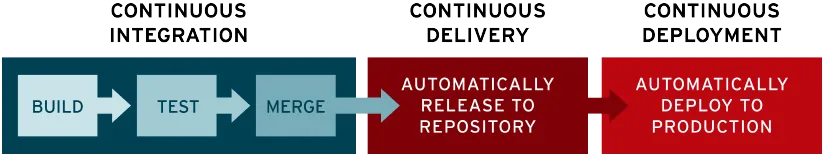
\includegraphics[width=\textwidth]{project/images/ci-cd-flow-desktop.png}
    \caption{DevOps practices.}
    \label{fig:devops-practices}
\end{figure}

\subsubsection{Continuous Integration}

Continuous integration (CI) is the practice of automating the integration of code changes from multiple contributors into a single software project. It’s a primary DevOps best practice, allowing developers to frequently merge code changes into a central repository where builds and tests then run. Automated tools are used to assert the new code’s correctness before integration. \cite{atlassian}

\subsubsection{Continuous Delivery}

Continuous delivery is an extension of continuous integration since it automatically deploys all code changes to a testing and/or production environment after the build stage.\cite{atlassian}

\subsubsection{Continuous Deployment}

Continuous deployment goes one step further than continuous delivery. With this practice, every change that passes all stages of your production pipeline is released to your customers. There's no human intervention, and only a failed test will prevent a new change to be deployed to production. \cite{atlassian}

\section{Testing Strategy}
The testing strategy outlines the approach that was adopted during the software testing process at SeekMake. It includes the testing objectives, scope, and resources required to carry out the testing activities.

\subsection{Testing Objectives}
The primary testing objectives were to ensure seamless user experiences by validating the core functionalities of SeekMake’s web application. Specific goals included verifying the checkout workflow, ensuring secure payment processing, and assessing the application’s compatibility across major browsers and devices.

\subsection{Testing Scope}
The testing scope included the following areas of the web application:

\begin{itemize}
    \item \textbf{Functionality:} Verify that the web application functions as expected.
    \item \textbf{Performance:} Evaluate the performance of the web application under different conditions.
    \item \textbf{Usability:} Assess the usability of the web application from an end-user perspective.
    \item \textbf{Compatibility:} Test the web application on different devices and browsers to ensure compatibility.
    \item \textbf{Security:} Identify and address security vulnerabilities in the web application.
\end{itemize}

\subsection{Testing Resources}
The testing resources required to carry out the testing activities included the following:

\begin{itemize}
    \item \textbf{QA Testers:} QA testers responsible for designing, executing, and reporting test cases.
    \item \textbf{Developers:} Developers responsible for fixing defects identified during testing.
    \item \textbf{Product Owner:} Product owner responsible for defining the requirements and acceptance criteria.
    \item \textbf{Scrum Master:} Scrum master responsible for facilitating the testing process and ensuring that the testing activities are aligned with the sprint goals.
    \item \textbf{Test Environment:} Test environments including production, staging, and development environments to test the web application in different scenarios.
    \item \textbf{Testing Tools:} Testing tools including GitHub, Playwright, Microsoft Teams, BrowserStack Live, and Lighthouse to manage the testing process, automate testing activities, and track defects.
    \item \textbf{Documentation:} Test plans, test cases, test reports, and defect reports to document the testing activities and results.
    \item \textbf{Communication:} Regular communication between team members to share updates, collaborate on testing activities, and resolve issues.
    \item \textbf{Training:} Training sessions to familiarize team members with the testing tools and techniques used during the testing process.
    \item \textbf{Feedback:} Feedback sessions to provide continuous feedback on the testing process and identify areas for improvement.
\end{itemize}

\section{Testing Types}

A lot of test types exist and can be applied in projects \cite{istqbctfl4.0.1}. During this internship, the following three test types are
addressed:

\subsection{Functional Testing}
Functional testing evaluates the functions that a component or system should perform. The functions
are “what” the test object should do. The main objective of functional testing is checking the functional
completeness, functional correctness and functional appropriateness. \cite{istqbctfl4.0.1}

At SeekMake, functional testing was carried out to evaluate the functionality of the web application.
\subsection{Non-Functional Testing}
Non-functional testing evaluates attributes other than functional characteristics of a component or
system. Non-functional testing is the testing of “how well the system behaves”. The main objective of non-
functional testing is checking the non-functional quality characteristics. \cite{istqbctfl4.0.1}

At SeekMake, non-functional testing was carried out to evaluate the performance, usability, compatibility, and security of the web application.
\subsection{Black-box Testing}
Black-box testing is specification-based and derives tests from documentation not
related to the internal structure of the test object. The main objective of black-box testing is checking the
system's behavior against its specifications. \cite{istqbctfl4.0.1}

At SeekMake, black-box testing was carried out to evaluate the functionality of the web application from an end-user perspective.
\section{Testing Tools}
Various testing tools were used during the software testing process at SeekMake.
\subsection{GitHub, GitHub Actions and GitHub Projects}
\subsubsection{GitHub}
GitHub is a cloud-based platform where you can store, share, and work together with others to write code. \cite{github}

Collaborative working, one of GitHub’s fundamental features, is made possible by the open-source software, Git, upon which GitHub is built. \cite{github}

Git is a version control system that intelligently tracks changes in files. Git is particularly useful when you and a group of people are all making changes to the same files at the same time. \cite{github}


At SeekMake, GitHub was used to store the source code in repositories, manage branches, and collaborate on code changes.

\begin{figure}[H]
    \centering
    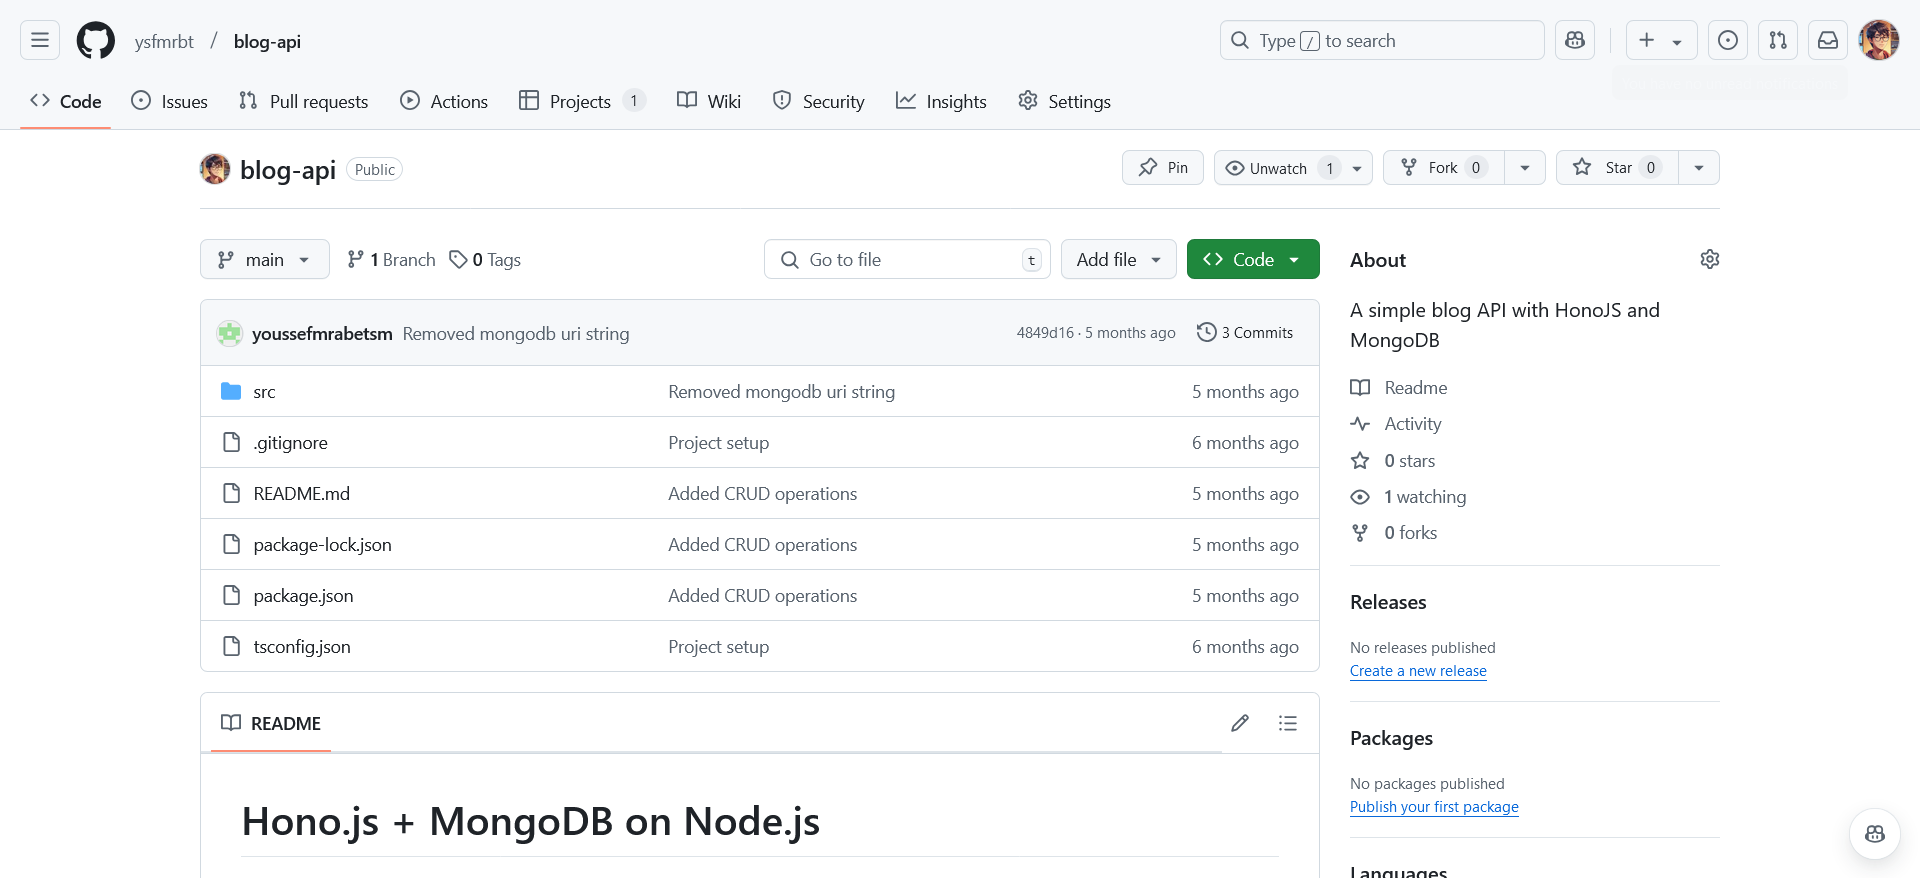
\includegraphics[width=\textwidth]{project/images/repo.png}
    \caption{An example of a GitHub repository.}
    \label{fig:github-repo}
\end{figure}
\subsubsection{GitHub Actions}
GitHub Actions is a continuous integration and continuous delivery (CI/CD) platform that allows you to automate your build, test, and deployment pipeline. \cite{ghactions}

GitHub Actions automated the execution of Playwright scripts, providing immediate feedback on code changes during sprints.

\begin{figure}[H]
    \centering
    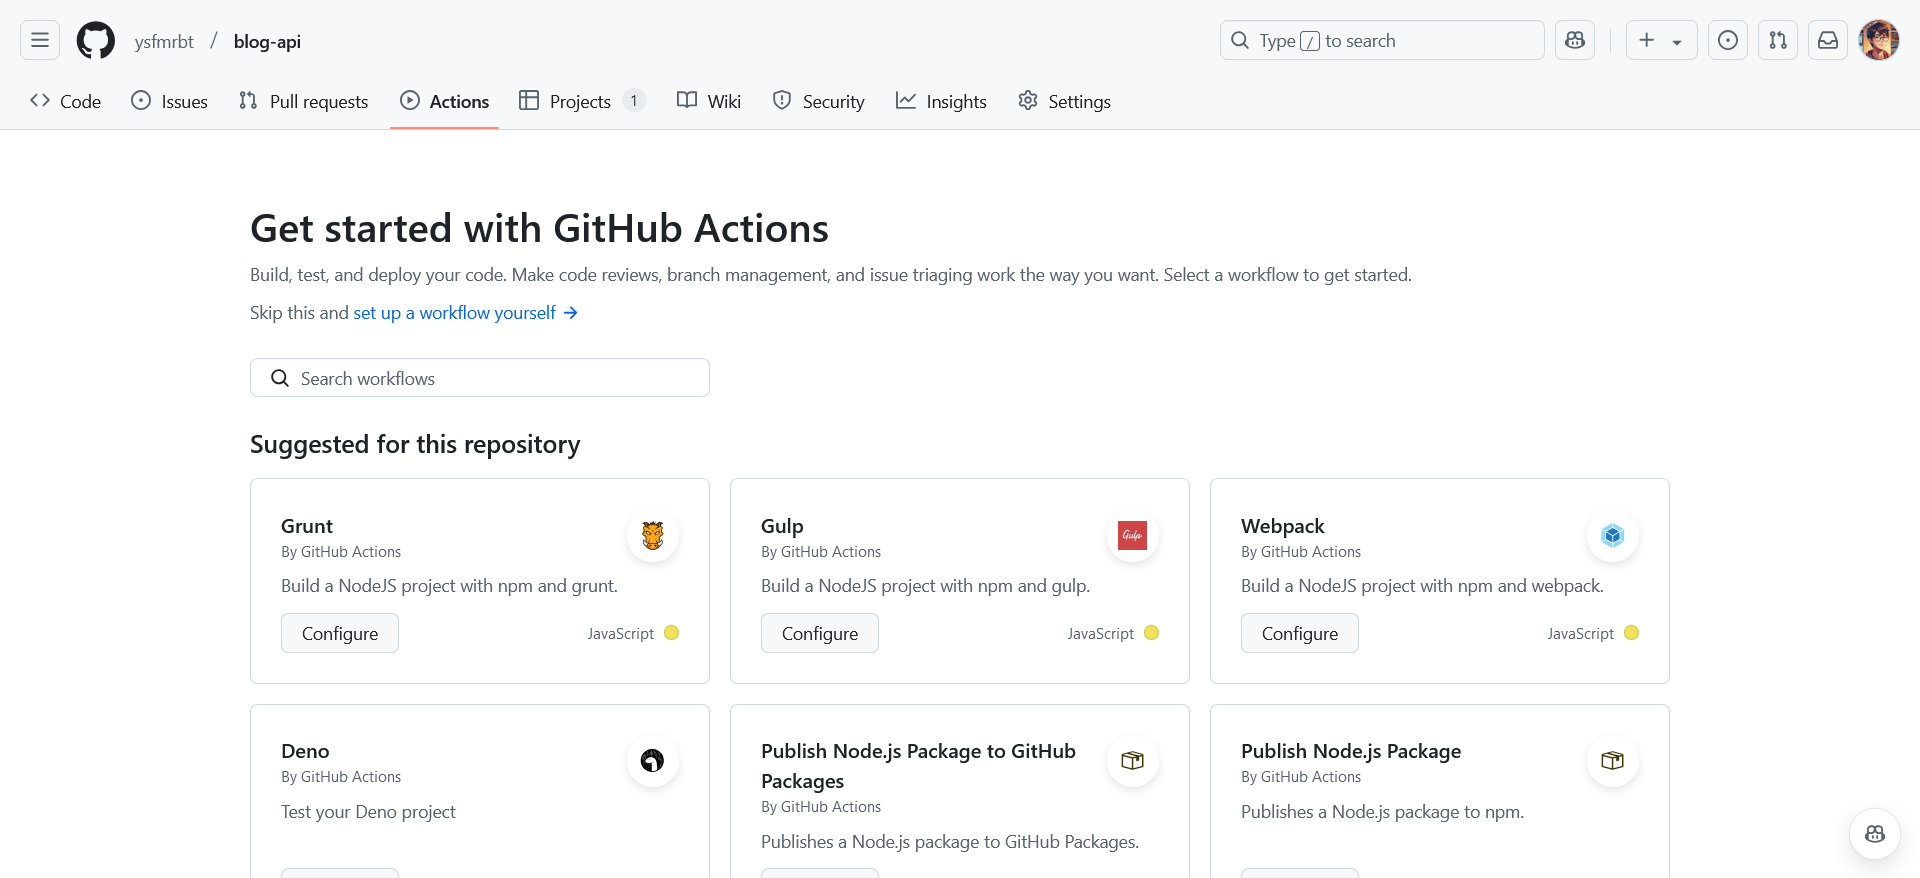
\includegraphics[width=\textwidth]{project/images/actions.png}
    \caption{GitHub Actions.}
    \label{fig:github-actions}
\end{figure}

\subsubsection{GitHub Projects}
Projects is an adaptable, flexible tool for planning and tracking work on GitHub. \cite{ghprojects}

At SeekMake, GitHub Projects was used to manage the testing process, track defects, and collaborate on testing activities.

\begin{figure}[H]
    \centering
    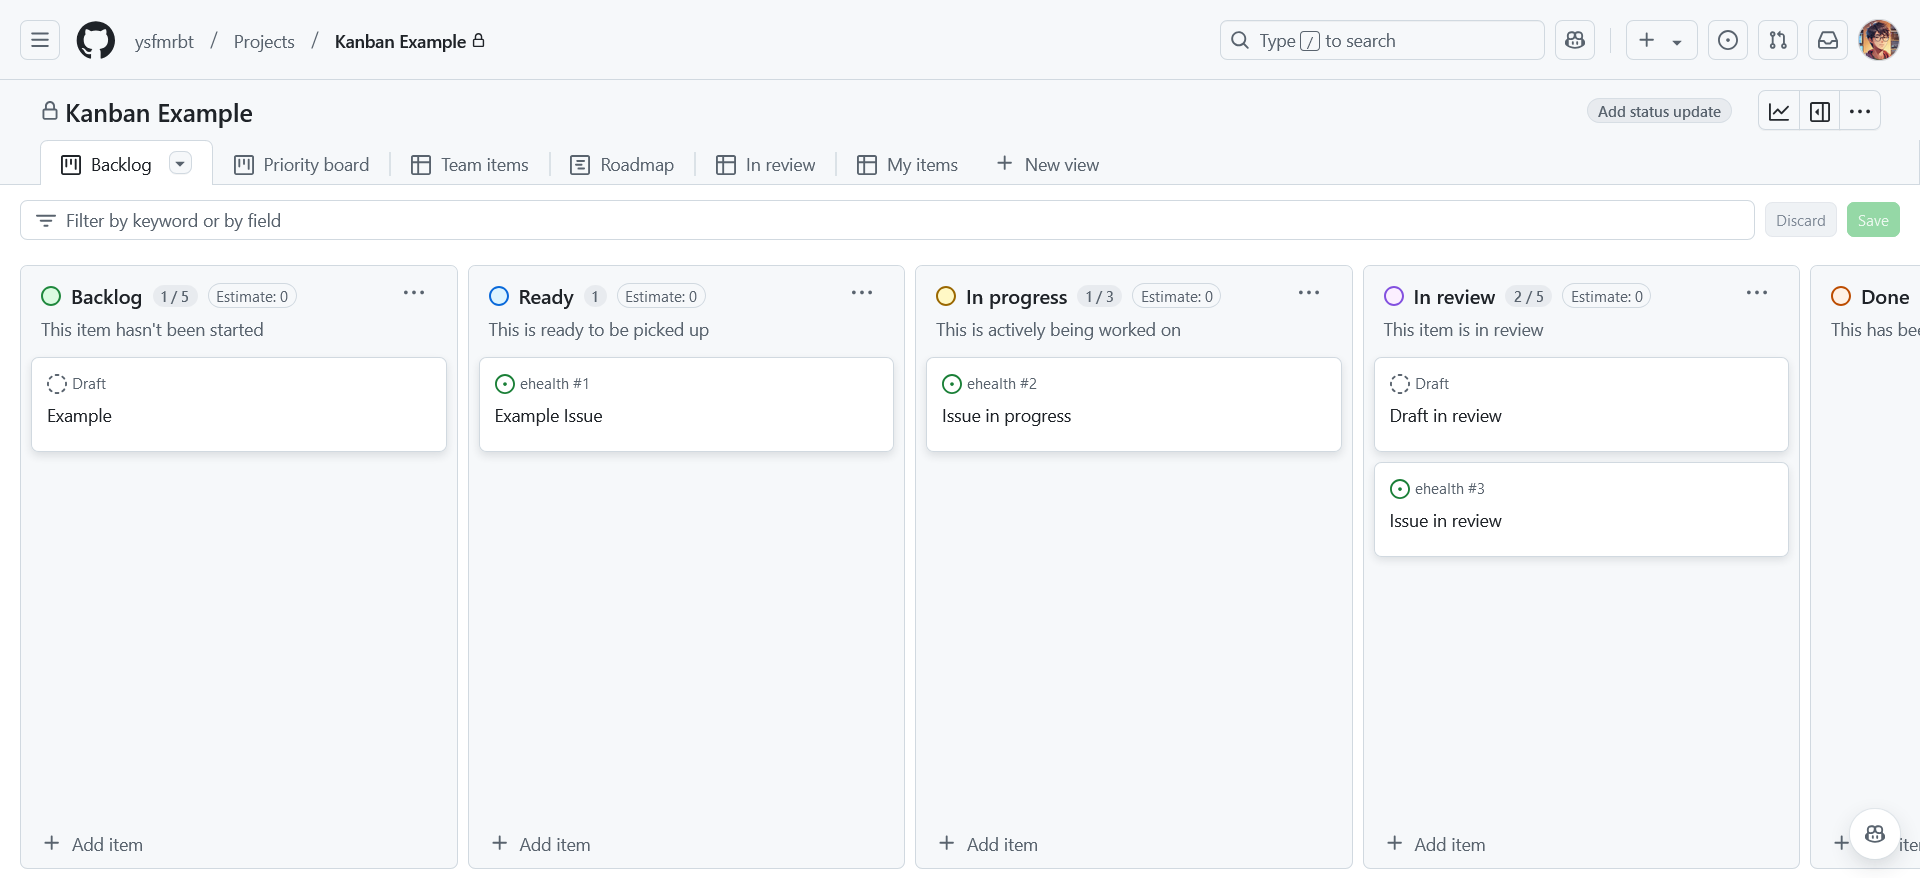
\includegraphics[width=\textwidth]{project/images/kanban.png}
    \caption{A GitHub project board resembling the Kanban board used at SeekMake.}
    \label{fig:github-kanban}
\end{figure}

\subsection{Playwright}
Playwright is a testing framework that enables reliable end-to-end testing for modern web apps \cite{pwhp}. It was created specifically to accommodate the needs of end-to-end testing. Playwright supports all modern rendering engines including Chromium, WebKit, and Firefox. Test on Windows, Linux, and macOS, locally or on CI, headless or headed with native mobile emulation. \cite{pwdocs}

Playwright was used for end-to-end testing, enabling automation across Chromium, WebKit, and Firefox browsers. It streamlined test execution for critical paths, such as the login process and account management workflows.

\begin{figure}[H]
    \centering
    
\includegraphics[width=0.5\textwidth]{project/images/Playwright_Logo.svg.png}
    \caption{Playwright logo.}
    \label{fig:playwright-logo}
\end{figure}

\subsection{Microsoft Teams}
Microsoft Teams is a Meet, chat, call, and collaborate with communications software that makes it easy to work, plan, and innovate together. \cite{msteams}

At SeekMake, Microsoft Teams was used to communicate with team members, share updates, and collaborate on testing activities.

\begin{figure}[H]
    \centering
    \includegraphics[width=0.1\textwidth]{project/images/Microsoft_Office_Teams_(2018–present).svg.png}
    \caption{Microsoft Teams logo.}
    \label{fig:msteams-logo}
\end{figure}

\subsection{BrowserStack Live}
BrowserStack Live is a cross browser on desktop and mobile testing platform. \cite{browserstack}

At SeekMake, BrowserStack Live was used to test the web application on Apple devices.

\begin{figure}[H]
    \centering
    
\includegraphics[width=0.5\textwidth]{project/images/BrowserStack_idTaghUsQq_1.png}
    \caption{Browser Stack logo.}
    \label{fig:browserstack-logo}
\end{figure}

\subsection{Lighthouse}

Lighthouse is an open-source, automated tool to help you improve the quality of web pages. You can run it on any web page, public or requiring authentication. It has audits for performance, accessibility, progressive web apps, SEO, and more.

At SeekMake, Lighthouse was used to assess web application performance and highlight areas for improvement, such as load times and accessibility.

\begin{figure}[H]
    \centering
    
\includegraphics[width=0.1\textwidth]{project/images/lighthouse-logo_512px.png}
    \caption{Lighthouse logo.}
    \label{fig:lighthouse-logo}
\end{figure}

\section{Testing Techniques}

Test techniques support the tester in test analysis (what to test) and in test design (how to test). Test
techniques help to develop a relatively small, but sufficient, set of test cases in a systematic way. Test
techniques also help the tester to define test conditions, identify coverage items, and identify test data
during the test analysis and design. \cite{istqbctfl4.0.1}

At SeekMake, the following testing techniques were used to design test cases:

\subsection{Black-box Testing Techniques}
Black-box test techniques (also known as specification-based techniques) are based on an analysis of
the specified behavior of the test object without reference to its internal structure. Therefore, the test
cases are independent of how the software is implemented. Consequently, if the implementation
changes, but the required behavior stays the same, then the test cases are still useful. \cite{istqbctfl4.0.1}

\subsubsection{Equivalence Partitioning}
Equivalence Partitioning (EP) divides data into partitions (known as equivalence partitions) based on the
expectation that all the elements of a given partition are to be processed in the same way by the test
object. The theory behind this technique is that if a test case, that tests one value from an equivalence
partition, detects a defect, this defect should also be detected by test cases that test any other value from
the same partition. Therefore, one test for each partition is sufficient. \cite{istqbctfl4.0.1}

At SeekMake, we used equivalence partitioning to design and execute test cases that verify discounts based on intervals of quantities.

\begin{figure}[H]
    \centering
    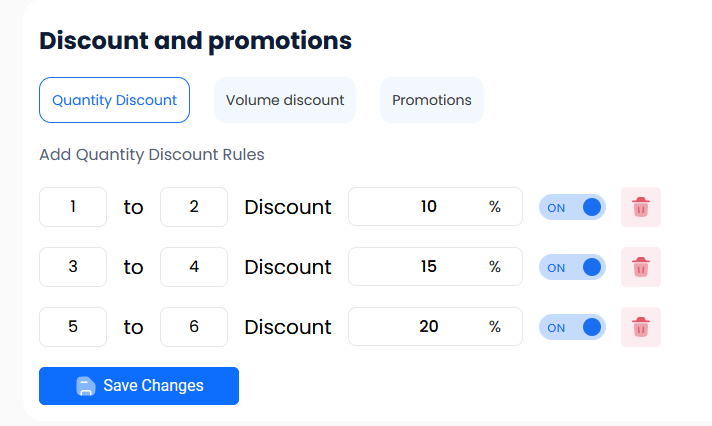
\includegraphics[width=0.5\textwidth]{project/images/ep.png}
    \caption{Screenshot taken from SeekMake's web application showing discounts based on intervals of quantities.}
    \label{fig:ep}
\end{figure}

\subsubsection{Boundary Value Analysis}
Boundary Value Analysis (BVA) is a test technique based on exercising the boundaries of equivalence
partitions. Therefore, BVA can only be used for ordered partitions. The minimum and maximum values of
a partition are its boundary values. In the case of BVA, if two elements belong to the same partition, all
elements between them must also belong to that partition. \cite{istqbctfl4.0.1}

At SeekMake, we used boundary value analysis to design and execute test cases that verify the behavior of the web application when the percentage of VAT is at the minimum and maximum values.

\begin{figure}[H]
    \centering
    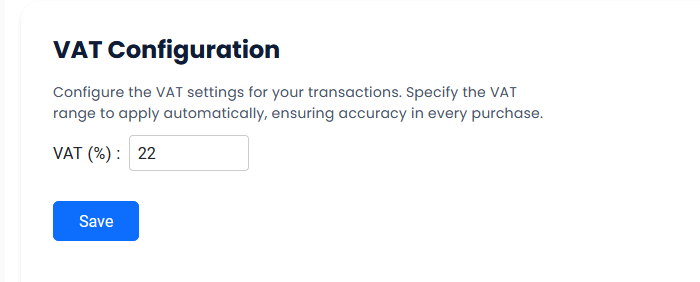
\includegraphics[width=0.5\textwidth]{project/images/bva.png}
    \caption{Screenshot taken from SeekMake's web application showing the percentage of VAT.}
    \label{fig:bva}
\end{figure}

\subsection{Experience-based Testing Techniques}
Experience-based test techniques effectively use the knowledge and experience of testers for the
design and implementation of test cases. The effectiveness of these test techniques depends heavily on
the tester’s skills. Experience-based test techniques can detect defects that may be missed using the
black-box test techniques and white-box test techniques. Hence, experience-based test techniques are
complementary to the black-box test techniques and white-box test techniques. \cite{istqbctfl4.0.1}

\subsubsection{Exploratory Testing}
In exploratory testing, tests are simultaneously designed, executed, and evaluated while the tester learns
about the test object. The testing is used to learn more about the test object, to explore it more deeply
with focused tests, and to create tests for untested areas. \cite{istqbctfl4.0.1}

At SeekMake, exploratory testing was carried out while we were learning about the web application and exploring its functionalities.
\subsubsection{Checklist-based Testing}
In checklist-based testing, a tester designs, implements, and executes tests to cover test conditions from
a checklist. Checklists can be built based on experience, knowledge about what is important for the user,
or an understanding of why and how software fails. Checklists should not contain items that can be
checked automatically, items better suited as entry criteria, exit criteria, or items that are too general
(Brykczynski 1999). \cite{istqbctfl4.0.1}

\begin{figure}[H]
    \centering
    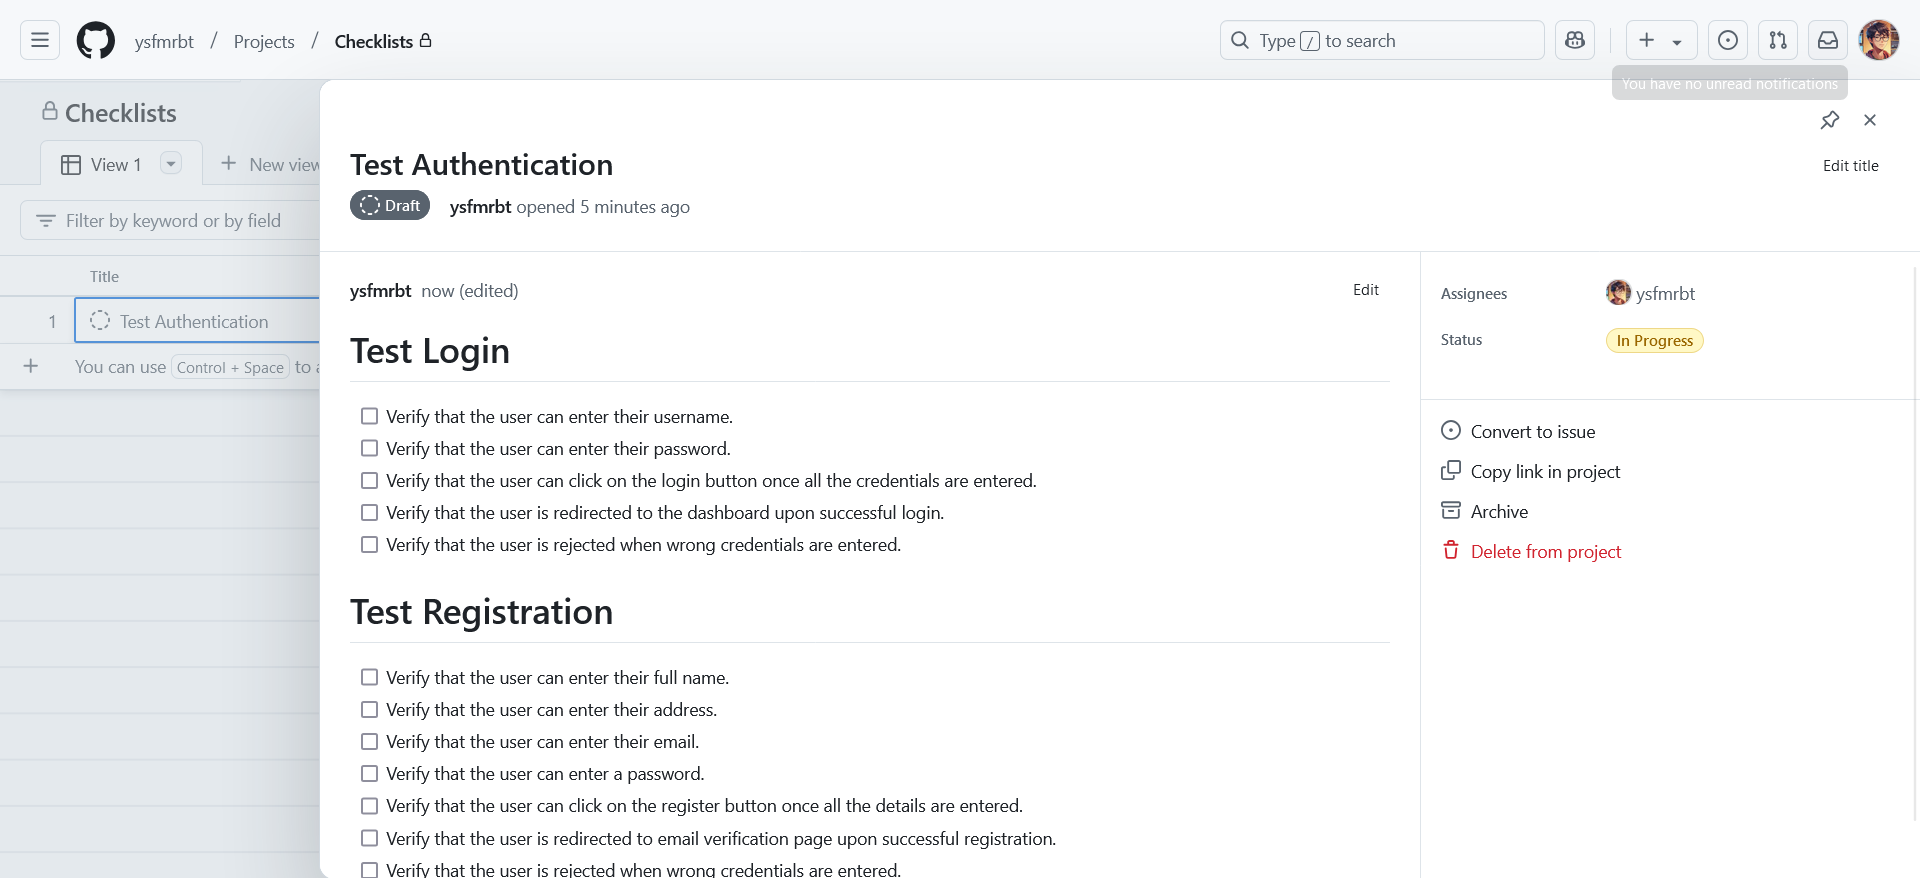
\includegraphics[width=\textwidth]{project/images/checklist.png}
    \caption{An example checklist used for Checklist-based testing at SeekMake.}
    \label{fig:gh-checklist}
\end{figure}

At SeekMake, checklist-based testing was carried out to ensure that all test conditions were covered during the testing process. We used the insights gained from exploratory testing to create checklists for future testing activities.

\section{Summary}
This chapter presented the methodology used during the software testing process at SeekMake. It included the testing strategy, testing types, testing tools, and testing techniques used to ensure the quality of the software.

The testing process was aligned with the Scrum methodology, and various testing tools were used to manage the testing process, automate testing activities, and track defects.

The testing techniques used to design test cases included black-box testing techniques and experience-based testing techniques.

The testing activities were carried out in parallel with the development activities to ensure that the software was thoroughly tested before each release.

In the next chapters, we will present how the sprints were carried out during the internship, the testing activities performed, and the results obtained.